\documentclass[oneside,final,14pt,a4paper]{extreport}

\usepackage{tempora} % Times New Roman alike font

\usepackage{vmargin}
\setpapersize{A4}
\setmarginsrb{2.5cm}{2.2cm}{2.2cm}{2.2cm}{0pt}{10mm}{0pt}{13mm}
\usepackage{setspace}
\setstretch{1.5}
\usepackage{indentfirst}
\parindent=1.25cm

%%%%% ADDED TO SUPPORT TT BOLD FACES %%%%
\DeclareFontShape{OT1}{cmtt}{bx}{n}{<5><6><7><8><9><10><10.95><12><14.4><17.28><20.74><24.88>cmttb10}{}
\renewcommand{\ttdefault}{pcr}
%%%%% END %%%%%%%%%%%%%%%%%%%%%%%%%%%%%%%

\usepackage{atbegshi,picture}
\usepackage[T1,T2A]{fontenc}
\usepackage[utf8]{inputenc}
\usepackage{fontspec}
\setmainfont{Times New Roman}

\usepackage[english]{babel}
\usepackage[backend=biber,style=ieee,autocite=inline]{biblatex}
\setcounter{biburlnumpenalty}{9000}
\setcounter{biburllcpenalty}{9000}
\setcounter{biburlucpenalty}{9000}
\bibliography{ref.bib}
\DefineBibliographyStrings{english}{%
  bibliography = {References},}
\usepackage{blindtext}

\usepackage{pdfpages}
\newenvironment{bottompar}{\par\vspace*{\fill}}{\clearpage}
\usepackage{amsmath,amsfonts}
\usepackage{url}
\usepackage{amsthm}
\newtheorem{theorem}{Theorem}
\newtheorem{corollary}{Corollary}
\newtheorem{lemma}{Lemma}
\newtheorem{proposition}{Proposition}
\theoremstyle{definition}
\newtheorem{definition}{Definition}
\theoremstyle{remark}
\newtheorem*{remark}{Remark}
\theoremstyle{remark}
\newtheorem*{example}{Example}

\usepackage{float}
\usepackage{graphicx}
\graphicspath{{figs/}} %path to images
\usepackage{array}
\usepackage{multirow,array}
\usepackage{caption}
\usepackage{subcaption}
\usepackage[unicode, colorlinks=true, linkcolor=black, urlcolor=black, citecolor=black]{hyperref}
\usepackage{paralist}
\usepackage{listings}
\usepackage{zed-csp}
\usepackage{fancyhdr}
\usepackage{csquotes}
\usepackage{color}
\usepackage{xcolor}
\definecolor{LightGray}{gray}{0.9}
\usepackage[outputdir=out]{minted}
\setminted{
  frame=lines,
  framesep=2mm,
  baselinestretch=1.2,
  bgcolor=LightGray,
  fontsize=\footnotesize,
  linenos
}
% \usepackage{anyfontsize}
% \usepackage{mathptmx}
% \usepackage{t1enc}

\usepackage{chngcntr}
\usepackage{upgreek}
\usepackage{bm}
\usepackage{hyperref}
\usepackage{booktabs}
\usepackage{multirow}
\usepackage{longtable}
\usepackage[font=singlespacing, labelfont=bf]{caption}
%Hints
\newcommand\pic[1]{(Fig. \ref{#1})} %Ref on figure
\newcommand\tab[1]{(Tab. \ref{#1})} %Ref on table

\setlength{\headheight}{32.0976pt}
\usepackage{enumitem}
\newlist{inlinelist}{enumerate*}{1}
\setlist*[inlinelist,1]{%
  label=(\arabic*),
}

% \setcounter{secnumdepth}{4}
\captionsetup[table]{labelfont={normalfont}, name={TABLE}, labelsep={newline}}
\setlength{\parindent}{2em}
\DeclareCaptionLabelSeparator{figSep}{.\quad}
\captionsetup[figure]{labelfont={normalfont}, name={Fig.}, labelsep=period}
\counterwithout{figure}{chapter}

% \usagepackage{titlesec}
% \titleformat{\section}[hang]{\fontsize{20}{24}\selectfont\filcenter}{\Roman{section}}{1em}{}
% \titleformat{\subsection}[hang]{\itshape}{\Alph{subsection}.}{1em}{}[]
% \titleformat{\subsubsection}[runin]{\itshape}{\arabic{subsubsection})}{1em}{}[$:$]
% \titlespacing{\subsubsection}{1em}{1em}{1em}
% \titleformat{\paragraph}[runin]{\itshape}{\alph{paragraph})}{1em}{}[$:$\quad]
% \titlespacing{\paragraph}{2em}{1em}{1em}

\usepackage{placeins} % for \FloatBarrier

\pagestyle{fancyplain}

% remember section title
\renewcommand{\chaptermark}[1]%
	{\markboth{\chaptername~\thechapter~--~#1}{}}

% subsection number and title
\renewcommand{\sectionmark}[1]%
	{\markright{\thesection\ #1}}

\rhead[\fancyplain{}{\bf\leftmark}]%
      {\fancyplain{}{\bf\thepage}}
\lhead[\fancyplain{}{\bf\thepage}]%
      {\fancyplain{}{\bf\rightmark}}
\cfoot{} %bfseries


\newcommand{\dedication}[1]
   {\thispagestyle{empty}

   \begin{flushleft}\raggedleft #1\end{flushleft}
}

\newcommand{\Rzk}{\textsc{Rzk}}

\begin{document}

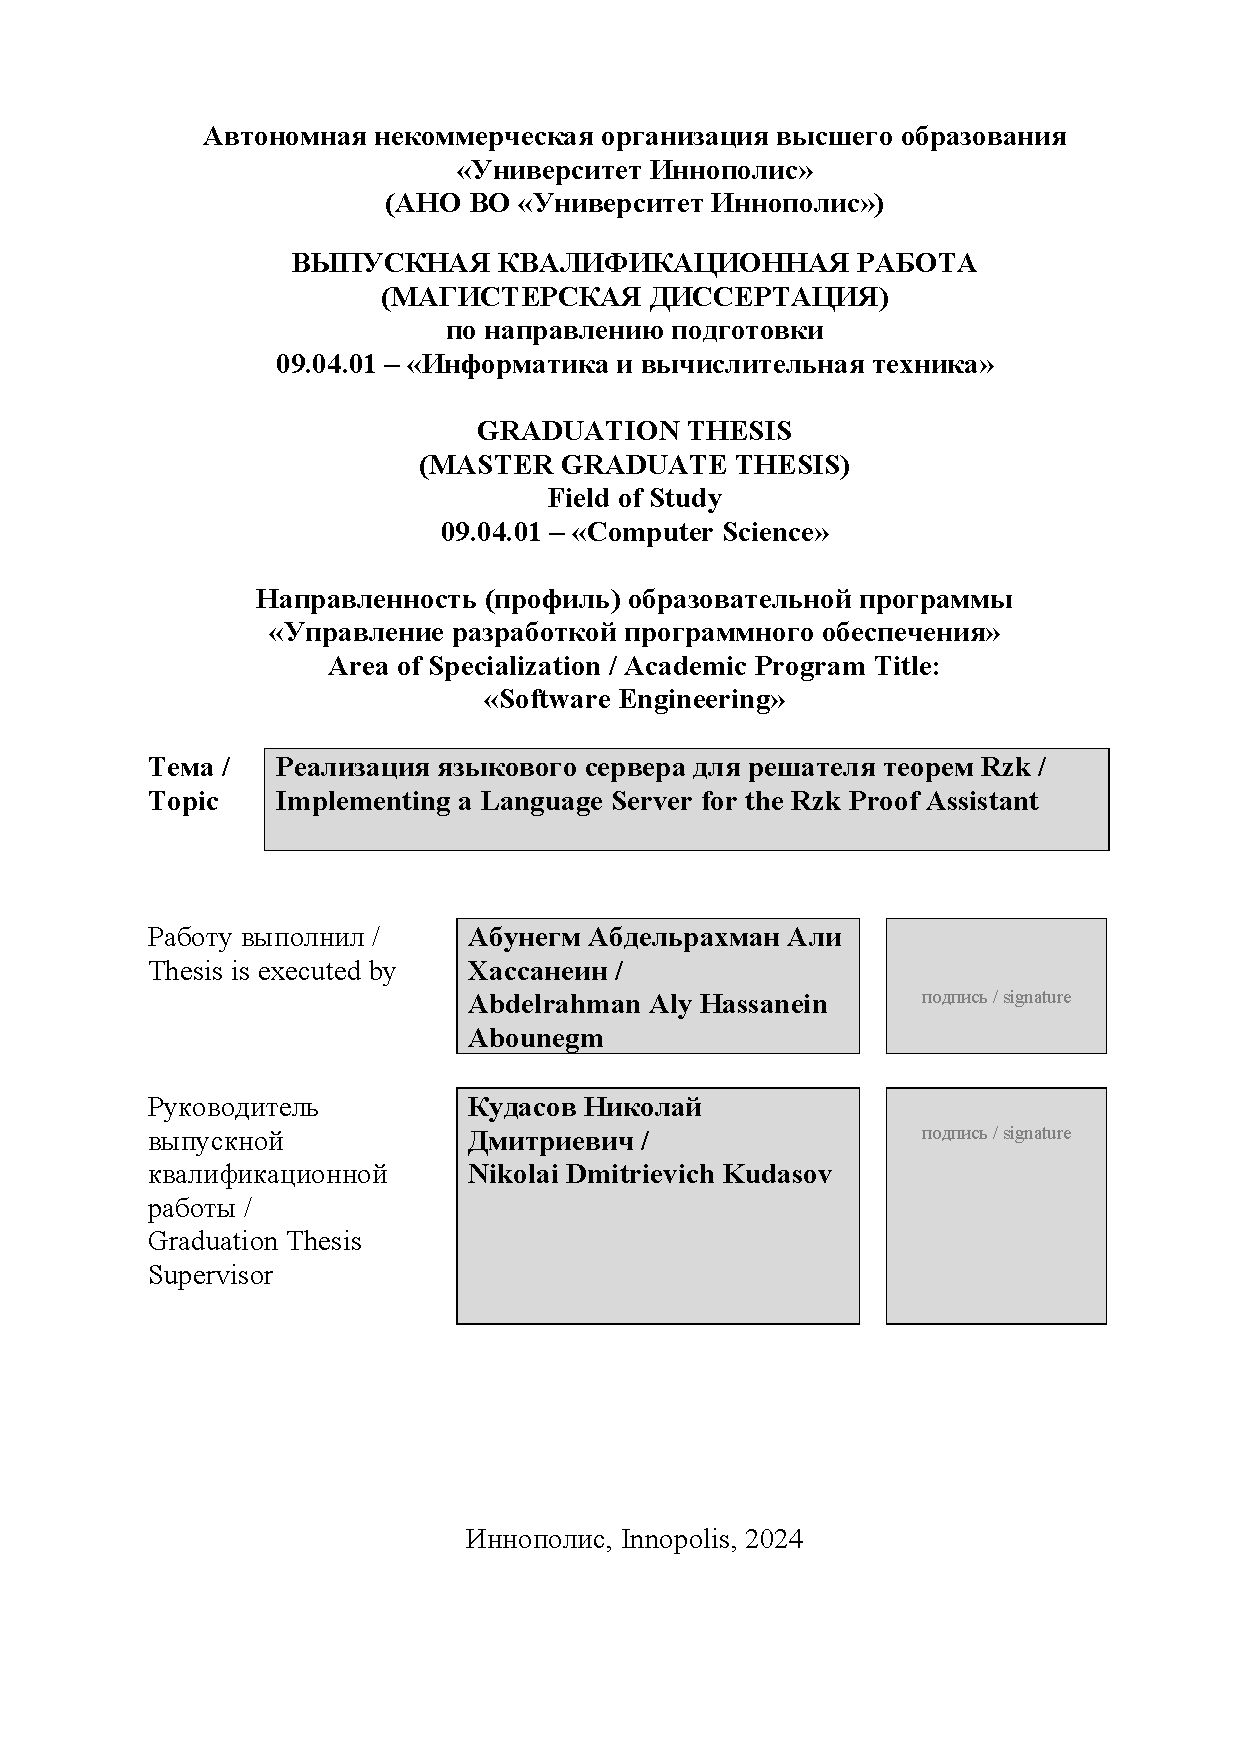
\includepdf[pages=-,offset={-\hoffset} {\voffset}]{title.pdf}
\tableofcontents
\listoffigures
\listoflistings
\newpage


\begin{abstract}
  The Riehl-Shulman type theory for synthetic $\infty$-categories is a new theory building on Homotopy Type Theory (HoTT).
  The experimental proof assistant \Rzk{} offers an automated proof checker for this theory.
  With the goal of making this theory more accessible to mathematicians and computer scientists,
  we present in this paper a work-in-progress on a collection of command line and interactive tools for \Rzk.
  These tools comprise a language server, an accompanying Visual Studio Code (VS Code) extension,
  and a list of smaller satellite tools offering minor conveniences.
  Although we focus on the support of VS Code,
  the language server is also compatible with other popular editors that support the Language Server Protocol (LSP),
  such as Emacs and Vim.

  % To support interactivity, we adjust the typechecker in \Rzk{} to work in an incremental fashion. In this paper, we present an initial version of a generic approach to the design of typecheckers that focus on LSP support. Building on top of this, we design and implement the language server for \Rzk. The language server offers advanced language features, including syntax and semantic highlighting, code completion, and diagnostics reporting. The VS Code extension complements the server with a user-friendly interface, facilitating interactive theorem proving and exploration of higher-dimensional structures.

  % Additional tools are developed along with the extension and language server to provide a pleasant experience outside the editor as well. These include a plugin to MkDocs that renders tope diagrams, a GitHub Action to type-check formalizations in Continuous integration environments, and a Pygments plugin for syntax highlighting \Rzk{} code blocks in LaTeX documents.

  % The effectiveness and usability of the language server and satellite tools is verified by \Rzk{} users coming from different backgrounds (mathematics, computer science, and software engineering), who use \Rzk{} to formalize theorems and provide feedback on their experience.
\end{abstract}

\setcounter{page}{7}
% set manually an actual number from which introduction starts!
% Why do we put 7 in this case?
% Title page - page 1
% Contents - page 2, page 3
% List of tables - page 4
% List of figures - page 5
% Abstract - page 6
% Chapter 1 - page 7
% In your thesis the counter number can be different, please count carefully and insert the corresponding number.

\chapter{Introduction}
\label{chap:intro}

\section{Proof Assistants}

Proof assistants, also known as interactive theorem provers (ITPs),
are software tools used in mathematics, computer science, and formal methods
to assist in the development and verification of mathematical proofs.
These tools play a crucial role in ensuring the correctness and reliability
of complex mathematical statements and software systems.
Examples of such tools include Agda~\cite{BoveDybjerNorell2009}, Coq~\cite{BertotCasteran2013}, and Lean~\cite{deMouraUllrich2021}.

Although similar in principal to typechecking in programming languages,
proof checking is normally seen as an interactive process between the mathematician and a proof assistant.
To this end, most proof assistants provide some interactive features either through specialized IDEs
(e.g. CoqIDE\footnote{\url{https://coq.inria.fr/refman/practical-tools/coqide.html}}),
integrating via Proof General~\cite{Aspinall2000}, or Visual Studio Code
(via the Language Server Protocol (LSP)~\cite{Gunasinghe2022}).
Most well-established proof assistants support several of these options.

\Rzk{}~\cite{Kudasov2023-github-rzk} is a new proof assistant that is based on Riehl-Shulman's type theory for synthetic $\infty$-categories~\cite{RiehlShulman2017}\cite{Riehl2023}.
The proof assistant is experimental but has been successfully used recently to formalize some fundamental results for $\infty$-categories,
including the $\infty$-categorical Yoneda lemma~\cite{Kudasov2023}.
However, \Rzk{} lacked most of the aforementioned features that are usually found in theorem provers, such as interactivity and syntax highlighting.
This paper reports on the implementation of utility and interactive tools around \Rzk{} proof assistant, focusing on the language server and VS Code extension support.
The goal is to provide a more user-friendly interface for \Rzk{} that would make it easier to use for both beginners and experienced users.

\section{Language Servers}

A few years ago, when a new code editor was introduced,
it needed to support the most popular programming languages,
and depended on plugins written specifically for this editor to support languages not built into the editor.
This led to a lot of repetitive work to provide useful language feature for the same language on multiple editors,
and an inconsistency between the provided language features on different editors.
The idea of language servers is Microsoft's attempt to solve this problem by standardizing a protocol for communication between a code editor (the client) and a background process (the server) that provides the language features for a certain language. This protocol is known as Language Server Protocol (LSP) \cite{Gunasinghe2022}. With LSP, a language author need only implement the server once and would automatically get language support on any editor that supports LSP. Likewise, an editor that supports LSP would automatically get language support for any programming language that has an LSP server. Examples for the language features in question include providing diagnostic messages, jumping to the location an identifier is introduced, text completion, semantic syntax highlighting, and much more.

\begin{figure}
  \centering
  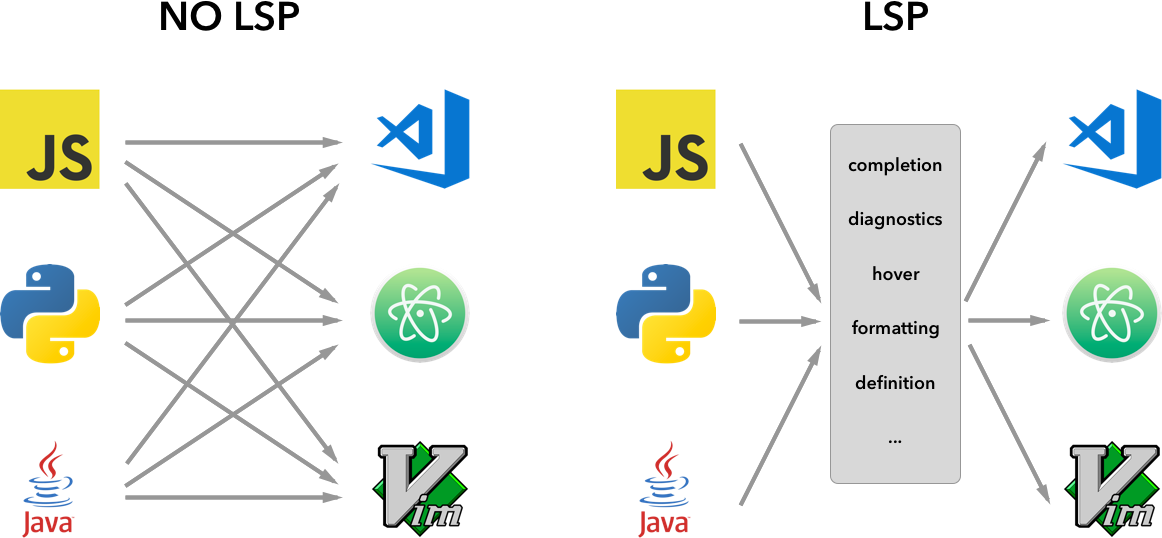
\includegraphics[width=0.7\textwidth]{figs/LSP-MxN.png}
  \label{figure:lsp}
  \caption{
    The motivation behind LSP, from Microsoft's website.
    \protect\footnotemark
  }
\end{figure}
\footnotetext{\raggedright\url{https://code.visualstudio.com/api/language-extensions/language-server-extension-guide}}

This protocol is particularly useful for interactive theorem provers since
they rely on the editing experience much more than a command line interface.
This is due to the fact that theorem provers generally do not need to compile
to any kind of executable file and only need the type-checking stage of compilers,
which can be easily performed by a language server. However, this also adds extra work
on the language server since it needs to support more features than a regular compiler would,
including listing variables in context along with their types, supporting Unicode symbols,
and most importantly allowing for an interactive step-by-step proof walkthrough.

\section{Contribution}

In this paper, we report on the work-in-progress on the implementation of
utility and interactive tools around \Rzk{} proof assistant, focusing on
the language server and VS Code extension support.

\chapter{Literature Review}
\label{chap:lr}
\chaptermark{Second Chapter Heading}

\section{Language Server Protocol}

The Language Server Protocol is a common protocol for programming language analyzers to communicate with development tools. The Language Server Protocol is used between a tool (the client) and a language smartness provider (the server) to integrate features like auto complete, go to definition, find all references and alike into the tool. The Language Server Protocol is used by many development tools like Visual Studio Code, Eclipse, Emacs, Sublime Text, Atom, and Vim. The Language Server Protocol is developed by Microsoft and is released under the Creative Commons Attribution License.

Its development started on June 27, 2016.
Microsoft collaborated with Red Hat and Codenvy to standardize the protocol's specifictation.
% https://www.infoworld.com/article/3088698/microsoft-backed-langauge-server-protocol-strives-for-language-tools-interoperability.html
% https://sdtimes.com/che/codenvy-microsoft-red-hat-collaborate-language-server-protocol/

\subsection{SLSP}

LSP is not good enough for "specification languages" (SL) because it is not designed for them. SLSP is a protocol for specification languages based on LSP.

It adds missing features (requests and notification types) for specification languages. It also adds a new feature for specification languages: "proof view" (a view of the proof state - like Lean's Info View).

% TODO: figure out what it uses DAP for exactly.

\section{Proof Assistants}

\chapter{System Requirements and Design}
\label{chap:req}

\chapter{Implementation}
\label{chap:impl}

\section{\Rzk{} Language Server and VS Code extesion}

In this section, we describe the implementation of the language server
and the VS Code extension for the \Rzk{} proof assistant.
The language server has direct access to the proof assistant internals,
including the typechecking algorithm and the internal abstract syntax representation,
and provides an interface conforming to the Language Server Protocol.
The VS Code extension then acts as a intermediary between the editor (VS Code)
and the language server, to bring the interactive capabilities to the user.

\subsection{Features}

% TODO: move this subsection to the requirements/design chapter?

We subject the language server to support the features specified below.

\subsubsection{Intuitive Interface and Syntax Highlighting.}

The VS Code extension introduces an intuitive interface that aligns with
the expectations of mathematicians and computer scientists.
Users benefit from clear and accessible navigation,
enabling efficient exploration of HoTT-based structures.
Furthermore, the extension provides syntax and semantic highlighting,
enhancing code readability, and facilitating error detection.

\begin{figure}
  \centering
  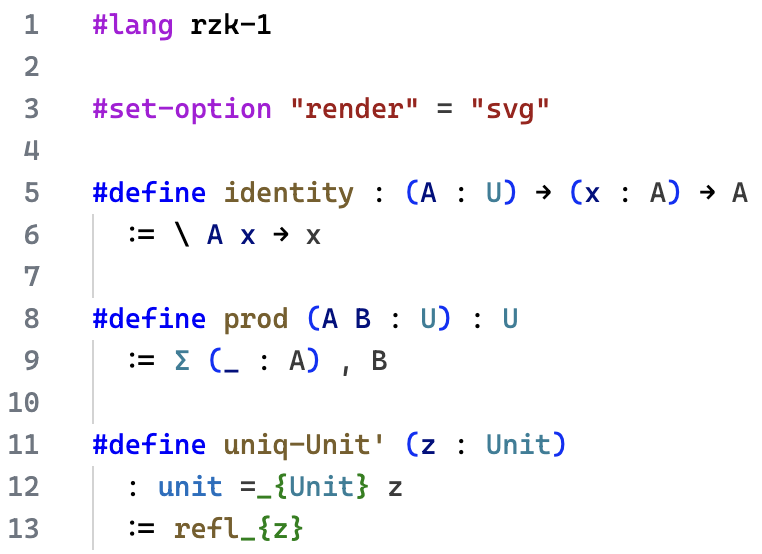
\includegraphics[width=0.7\textwidth]{figs/syntax-highlighting.png}
  \label{figure:syntax-highlighting}
  \caption{Syntax/Semantic highlighting in VS Code.}
\end{figure}

\subsubsection{Code Completion and Suggestions.}

\Rzk{}'s VS Code extension leverages the LSP to offer intelligent code completion
and context-aware suggestions. As users work with \Rzk{}, the extension assists
in writing code more efficiently by providing relevant suggestions, reducing
the likelihood of syntax errors, and accelerating the development process.

\begin{figure}
  \centering
  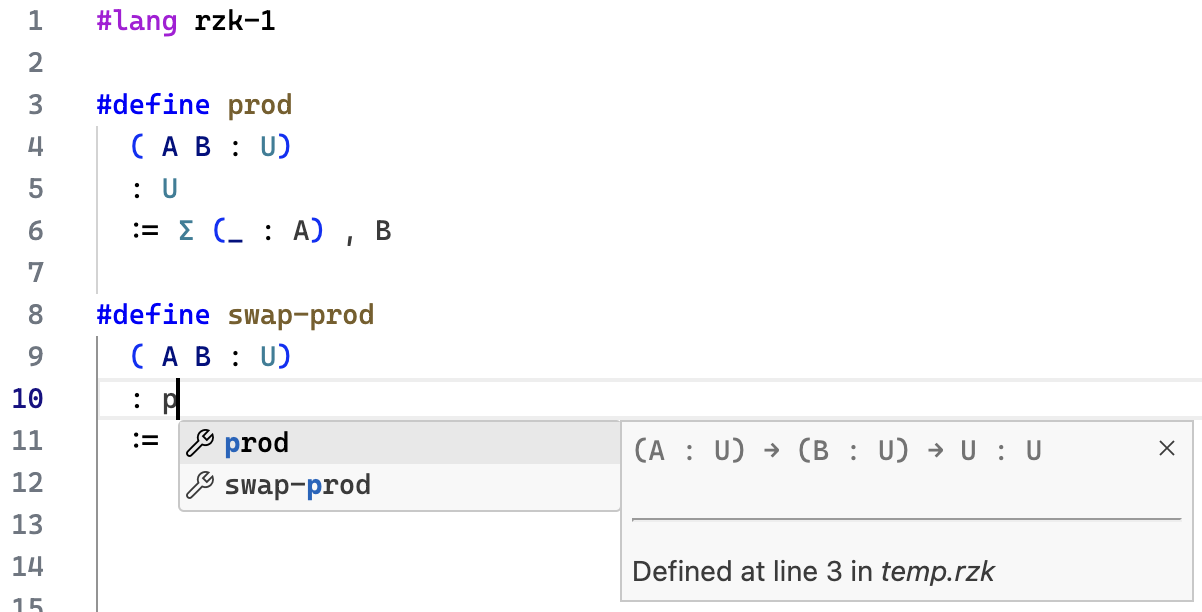
\includegraphics[width=0.7\textwidth]{figs/code-completions.png}
  \label{figure:code-completions}
  \caption{Code completions in VS Code.}
\end{figure}

\subsubsection{Real-time Error Checking.}

One of the extension's notable strengths lies in its ability to perform real-time error checking.
As users input and modify code, the language server continuously analyzes it,
reporting back any type errors or other issues with the proof.
This proactive error checking mechanism empowers users to identify and rectify issues promptly,
fostering the creation of mathematically sound programs.

\begin{figure}
  \centering
  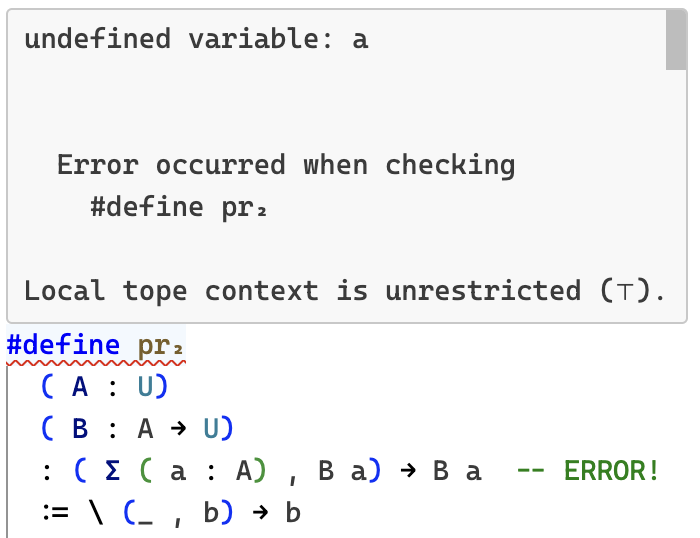
\includegraphics[width=0.7\textwidth]{figs/diagnostic-message.png}
  \label{figure:diagnostic-message}
  \caption{An error diagnostic message in VS Code.}
\end{figure}

\subsection{VS Code extension}

To bring about these features to the users, a thin wrapper around the language server in the form of a VS Code extension is necessary.
Additionally, the extension manages the installation of the language server itself on all major operating systems (Windows, macOS, and Ubuntu)
powered by pre-built binaries attached to releases on GitHub,
in addition to facilitating building the language server from source on platforms
for which pre-built binaries are not available.
The source code of the extension is available on the GitHub repository\footnote{
  \url{https://github.com/rzk-lang/vscode-rzk}},
and the extension itself is available on the Visual Studio Marketplace\footnote{
  \url{https://marketplace.visualstudio.com/items?itemName=NikolaiKudasovfizruk.rzk-1-experimental-highlighting}}.
and on the Open VSX registry\footnote{
  \url{https://open-vsx.org/extension/NikolaiKudasovfizruk/rzk-1-experimental-highlighting}},
as well as a pre-built binary on the GitHub releases page\footnote{
  \url{https://github.com/rzk-lang/vscode-rzk/releases}}.

\subsubsection{Installation and Activation}

Once the extension is activated, it checks if the \Rzk{} executable is available on the system's
\texttt{PATH} and if not, checks if it was previously downloaded to the extension's local storage directory.
If neither are available, it prompts the user to download the latest compatible binary from the GitHub
releases page and saves it in the local storage directory.
The user can override this behavior by specifying a custom path to the language server binary.

\begin{listing}
  \begin{minted}{typescript}
function locateRzk(context: vscode.ExtensionContext) {
  let path = vscode.workspace.getConfiguration().get<string>('rzk.path') ?? '';
  // Probe 1 - extension settings
  if (path) {
    const result = spawnSync(path, ['version']);
    if (result.status === 0) {
      return path;
    } else {
      output.appendLine(
        'The configured `rzk.path` option does not point to a valid rzk executable'
      );
    }
  }

  // Probe 2 - global PATH
  const binExtension = process.platform === 'win32' ? '.exe' : '';
  path = 'rzk' + binExtension;
  let result = spawnSync(path, ['version']);
  if (result.status === 0) {
    return path;
  } else {
    output.appendLine('Cannot find rzk globally');
  }

  // Probe 3 - extension storage bin folder
  path = vscode.Uri.joinPath(
    context.globalStorageUri,
    'bin',
    'rzk' + binExtension
  ).fsPath;
  result = spawnSync(path, ['version']);
  if (result.status === 0) { return path; }

  return null;
}
  \end{minted}
  \caption{The function responsible for finding where \Rzk{} is installed}
\end{listing}

To download a pre-built binary of \Rzk{}, the extension queries the available releases on the
GitHub repository and finds the latest release compatible with the installed version of the extension.
Compatibility is determined by defining a semver \cite{Preston2013semantic} range in the extension's source code,
which is then used to filter the releases and find the latest one that satisfies the range.

\begin{listing}
  \begin{minted}{typescript}
import semver from 'semver';
import type { RestEndpointMethodTypes } from '@octokit/rest';

/** In semver range format */
const supportedRzkVersions = '>=0.6.0 <1.0.0';

type GitHubRelease =
  RestEndpointMethodTypes['repos']['listReleases']['response']['data'][number];

/**
 * Checks whether the given rzk version is compatible with the extension
 * @param version A version string, e.g. "1.3.2" or "v0.4.1.1"
 */
export function isCompatibleVersion(version: string) {
  return semver.satisfies(semver.coerce(version) ?? '', supportedRzkVersions);
}
  \end{minted}
  \caption{Version compatibility check in the VS Code extension.}
  \label{code:ext-version}
\end{listing}

Then, the extension downloads the binary using Octokit SDK and extracts the tar archive to the local storage directory.

After that, the extension simply starts the language server in a separate process and establishes a connection to it,
and the rest is handled by VS Code and the language server.

\subsubsection{Configuration}

The extension provides configuration options to the user to customize the behavior of the extension.
The user can specify the path to the \Rzk{} executable, which is useful for users who have the executable installed in a non-standard location, as well as for testing purposes.
The user can also enable or disable the formatting feature and choose whether to receive pre-release versions of \Rzk{}.

\begin{figure}
  \centering
  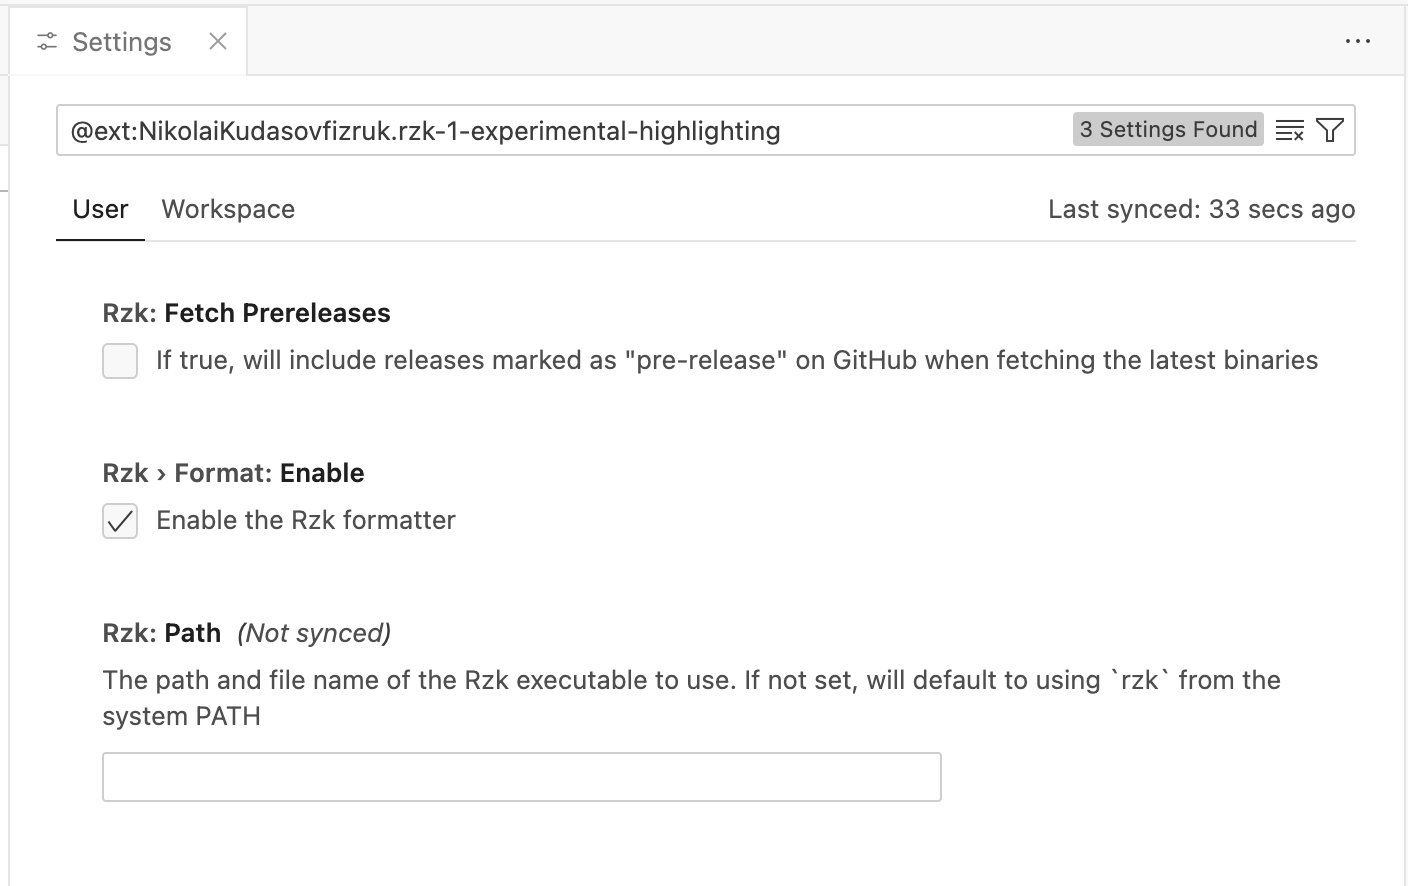
\includegraphics[width=0.8\textwidth]{figs/rzk-vscode-settings.png}
  \label{figure:vscode-settings}
  \caption{The extension configuration section in VS Code.}
\end{figure}

This is achieved using the configuration\footnote{
  \url{https://code.visualstudio.com/api/references/contribution-points\#contributes.configuration}}
field in \texttt{package.json}

\subsection{\Rzk{} Language Server}

At the core of the \Rzk{} tool suite is the language server that powers all the editor features that make it pleasant to develop proofs in \Rzk{}. In particular, it currently supports semantic highlighting, diagnostic messages, and text completion. Additionally, progress reporting for long-running processes (such as type-checking for large projects) is currently under work.

For the first versions of the language server, it is shipped as part of the \Rzk{} proof assistant itself under a different subcommand, but it is planned to decouple both components and have the language server depend on the core library. They are implemented in the Haskell programming language using the \texttt{lsp}\footnote{\url{https://hackage.haskell.org/package/lsp}} package.

It is also worth mentioning that the language server is designed to be compatible
with any other editor that supports LSP, not just VS Code.
In particular, users have reported success in integrating it with the NeoVim editor,
and it is planned to be tested with other editors as well.

The language server currently supports the features outlined in the following sections, with more features planned for the future.

\subsubsection{Diagnostics Reporting}

Every time the user saves a file that is part of a formalization project, the language server runs the typechecker
on the project and reports any errors or warnings that it finds, caching the results to speed up future typechecks.
The errors and warnings are sent as diagnostic messages via the LSP protocol to the editor,
which then displays them in the editor's interface.
This feature is crucial for the users to be able to quickly identify and fix any errors in their proofs.
These messages are displayed on the location in the file where the error occurred,
and contain a useful message that explains what went wrong with all the necessary context.

\subsubsection{Text Completion}

The language server also provides text completion suggestions to the user as they type.
These suggestions are context-aware and are based on the current cursor position in the file.
They include previously defined proof identifiers, their types, and their definition locations.

\subsubsection{Semantic Highlighting}

Another feature that the language server provides is semantic highlighting, which colors different parts of the code
based on their meaning.
This differs from syntax highlighting in that it is smarter and can use more information in determining a token's type (and hence color),
This is because it uses information from the parser, and not just from the lexer.
It can also use additional information from the typechecker to determine the type of a token,
but this is currently not implemented since it was not deemed necessary.

\subsubsection{Formatting}

The language server also provides a formatting feature that allows the user to format their code according to a predefined style.
This is useful for keeping the codebase consistent and readable, and is especially useful when working in a team.
The formatter catches common style issues such as indentation, spacing, and line breaks,
and automatically fixes them according to the predefined style.

A separate CLI subcommand is available to expose this feature outside of the language server as well.

\section{Satellite Tools}

% TODO

\subsection{MkDocs Plugin}

The \texttt{rzk-mkdocs-plugin} is a Python package that provides a plugin for the MkDocs static site generator.

\subsection{GitHub Action}

The \texttt{rzk-github-action} is a GitHub Action that can be used to run the \Rzk{} proof assistant on a GitHub repository.

\chapter{Evaluation and Discussion}
\label{chap:eval}

\chapter{Conclusion}
\label{chap:conclusion}

We have designed and implemented an initial prototype of the language server
and VS Code extension for an experimental proof assistant \Rzk{}.
An intermediate result of this work has been presented at the
\textit{Interactions of Proof Assistants and Mathematics}\footnote{\url{https://itp-school-2023.github.io/}}
school in Germany in September of 2023.
This has helped gather feedback from the users and react to it on the spot.
We feel that current users are mostly satisfied with the prototype tooling,
but have also provided useful suggestions for further improvements.

In the future, we plan to support displaying variable information on hover,
jumping to definition, renaming symbols, and formatting \Rzk{} code.
Eventually, we also plan to support rendering topes as images,
and adding an information WebView similar to the one provided by Lean 4 \cite{Nawrocki2023}.

It is also anticipated that a Haskell library for developing language servers
(especially for proof assistants) can grow out of this project.



%% REFERENCES
\printbibliography[heading=bibintoc,title={Bibliography cited}]
\appendix
\chapter{Extra Stuff}
\blindtext

\chapter{Even More Extra Stuff}
\blindtext

\end{document}
